\documentclass{report}
\usepackage{graphicx} % Required for inserting images
\usepackage[italian]{babel}
\usepackage{tikz}
\usepackage{hyperref}
\usepackage{amsmath}
\usepackage{xcolor}

\definecolor{darkgreen}{rgb}{0.0, 0.5, 0.0}


\title{Algoritmi per le Impronte Digitali}
\date{Parte IV}

\begin{document}

\maketitle

\tableofcontents
\newpage

\chapter{Algoritmi di prefiltraggio ed enhancement}


Nel modulo per \textbf{estrazione delle feature} si eseguono
tipicamente questi passi:
\begin{enumerate}
    \item filtraggio iniziale
    \item manipolazione dell'immagine (enhancement)
    \item estrazione delle feature
    \item codifica
\end{enumerate}

\begin{figure}[ht]
    \centering
    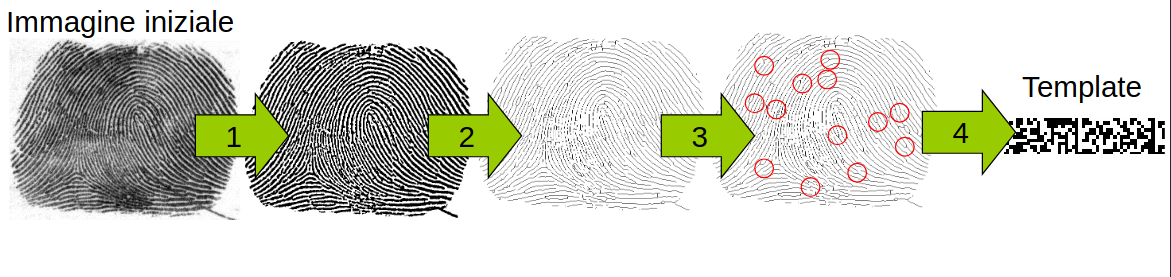
\includegraphics[width=1\linewidth]{images/estrazione-fet.png}
\end{figure}

In questa sezione ci concentriamo sui punti 1 e 2.

\newpage
\section{Filtraggi iniziali}

\subsection{Contrast streching}
Le immagini delle impronte digitali hanno di
solito una dinamica dei toni di grigio molto
limitata; l’operazione di Contrast Stretching allarga la
dinamica dell’immagine.

\begin{figure}[ht]
    \centering
    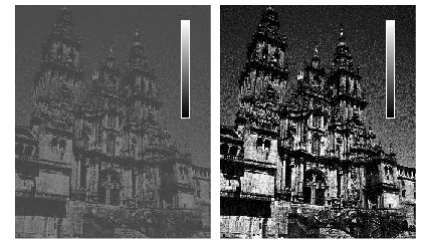
\includegraphics[width=0.5\linewidth]{images/constrast-stre.png}
\end{figure}

\subsection{Manipolazione dell'istogramma}

L’istogramma di una
immagine può essere
mappato in un altro
mediante diverse
funzioni; il logaritmo permette
ad esempio di
evidenziare delle
variazioni sottili di toni
di grigio in una
immagine che ha già
una dinamica elevata.

\begin{figure}[ht]
    \centering
    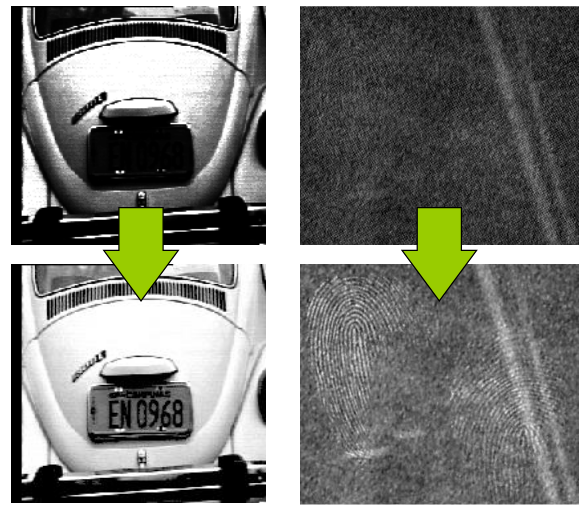
\includegraphics[width=0.5\linewidth]{images/man-isto.png}
\end{figure}

\newpage
\subsection{Filtro di Wiener}

Quando si conoscono le caratteristiche spettrali
dell’immagine e del rumore si usa il filtro di
Wiener. Si riesce a distinguire i rumori tra sfondo ed impronta, dando risalto al secondo.

\begin{figure}[ht]
    \centering
    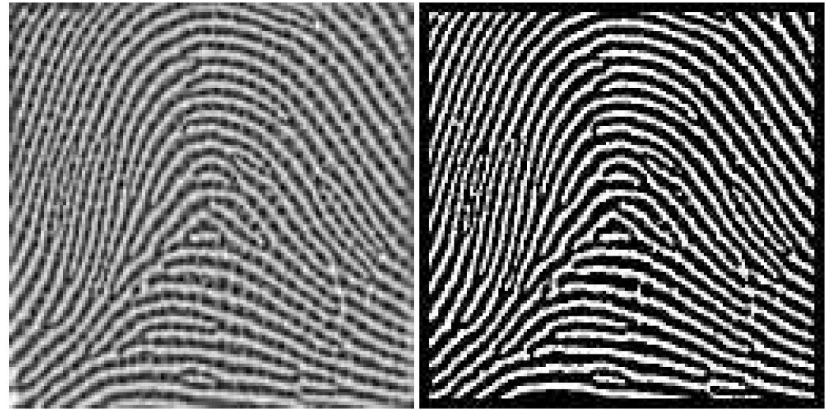
\includegraphics[width=0.5\linewidth]{images/filtro-we.png}
\end{figure}

\subsection{Normalizzazione}

L’obiettivo della normalizzazione è quello di standardizzare le
variazione di grigio dei ridge in tutta l’immagine per agevolare
gli algoritmi successivi.

\subsection{Segmentazione}

Gli algoritmi per la segmentazione estraggono il foreground
dal background (impronta dallo sfondo).

\begin{figure}[ht]
    \centering
    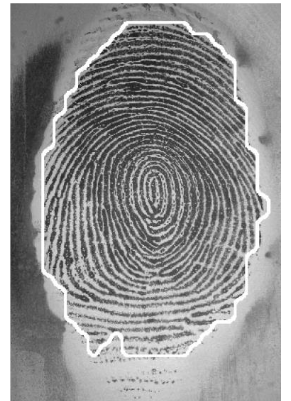
\includegraphics[width=0.3\linewidth]{images/segmentazione.png}
\end{figure}

\noindent Permettono di focalizzarsi solo sulle regioni della immagine che 
portano informazione utile al processo biometrico.

\subsection{Regioni con diversa qualità}

\noindent Una volta che l’impronta è stata individuata nella immagine
dalla segmentazione si iniziano le analisi successive.

\noindent Raramente una immagine di una impronta ha la stessa qualità
in tutte le regioni, a causa di:

\begin{itemize}
    \item diversa pressione
    \item traslazioni
    \item tagli
    \item uso non corretto dell'inchiostro
\end{itemize}

\noindent Di solito si distinguono tre regioni:
\begin{itemize}
    \item well-defined
    \item recoverable
    \item unrecovable
\end{itemize}

\section{Manipolazione dell'immagine (enhancement)}

Ha due obiettivi:
\begin{itemize}
    \item \textbf{migliorare la chiarezza della struttura dei ridge} dove possibile
    \item \textbf{marcare le regioni dove non è possibile estrarre informazione} perché c'è troppo rumore
\end{itemize}

\noindent Prende in ingresso una immagine di toni di grigio, e produce un'immagine 
a toni di grigio binarizzata.

\subsection{Filtri contestuali}

Per ottenere i massimi risultati nell‘evidenziare la
struttura dei ridge in una immagine occorre ricorrere ai
filtri adattativi o contestuali. Questa categoria dei filtraggi per le immagini modifica
automaticamente i propri parametri per meglio adattarsi
al mutare delle condizioni dell’immagine, basandosi su:
\begin{itemize}
    \item distanza tra i ridge
    \item orientamento dei ridge
    \item livello di rumore presente
\end{itemize}

\noindent Questi filtri lavorano sulla immagine in ingresso
attraverso un’operazione chiamata convoluzione con una
maschera di filtraggio.

\noindent A seconda del tipo di maschera usata il filtro
aumenta/diminuisce alcune caratteristiche piuttosto che
altre.

\begin{figure}[ht]
    \centering
    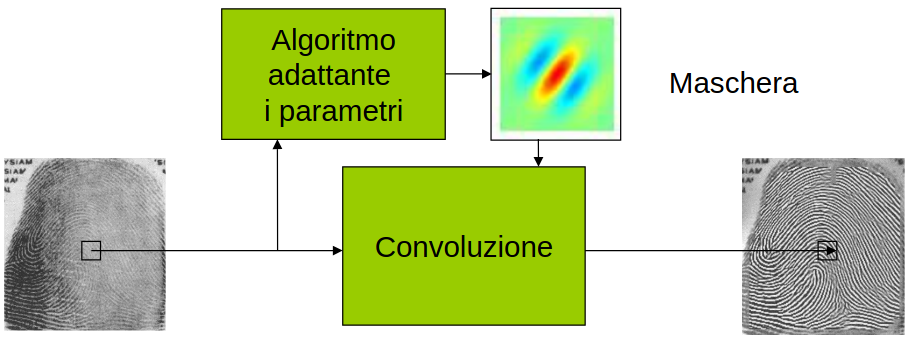
\includegraphics[width=0.6\linewidth]{images/filtro-contestuale.png}
\end{figure}

\newpage
\subsection{Filtro di O'Gorman e Nickerson}

La forma particolare di questa maschera è fatta per fare
“match” con lo spessore dei ridge, la loro distanza di
separazione, il valore del massimo e del minimo in un
intorno del punto di esame.

\noindent Questo filtro tende ad attenuare il rumore locale.


\chapter{Estrazione di caratteristiche}

\section{Caratteristiche di I livello}
In questa sezione ci concetriamo sull'estrazione delle feature di I livello (direzione dei ridge, core, delta, ridge count).

\subsection{Ridge counting}

E’ una misura dei ridge che attraversano una
linea immaginaria passante tra due minutiae.

\begin{figure}[ht]
    \centering
    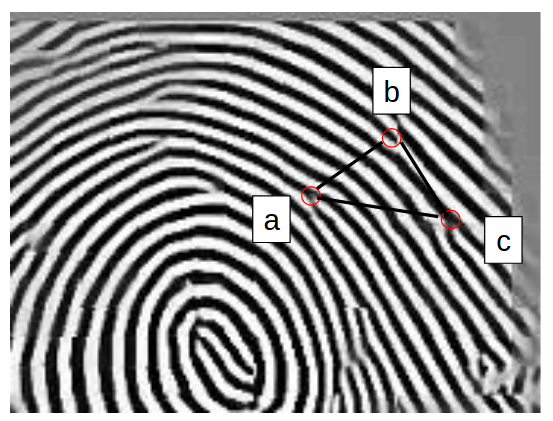
\includegraphics[width=0.5\linewidth]{images/ridge-counting.png}
\end{figure}

\begin{itemize}
    \item fra A e B 4 ridge
    \item fra B e C 0 ridge
    \item fra C e A 3 ridge
\end{itemize}

\newpage
\subsection{Analisi delle frequenze spaziali}

E’ una misura di quanto sono stretti o larghi i
ridge nelle varie regioni dell’impronta.

\begin{figure}[ht]
    \centering
    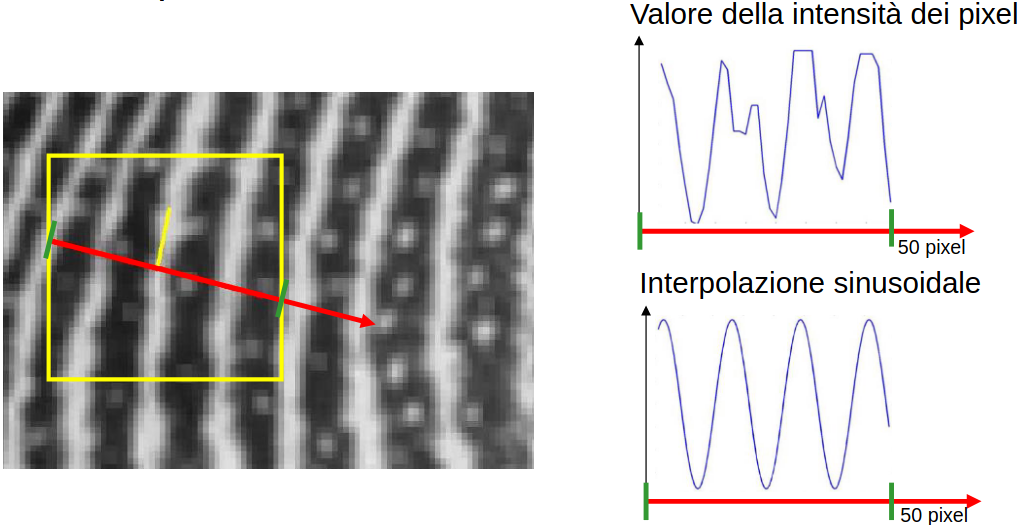
\includegraphics[width=1\linewidth]{images/ridge-freq.png}
\end{figure}

\subsubsection{Mappa delle frequenze spaziali}

Usando l’informazione ricavata dalle frequenze di
ridge per ogni blocco dell’immagine è possibile
avere la mappa delle frequenze dell’immagine.

\begin{figure}[ht]
    \centering
    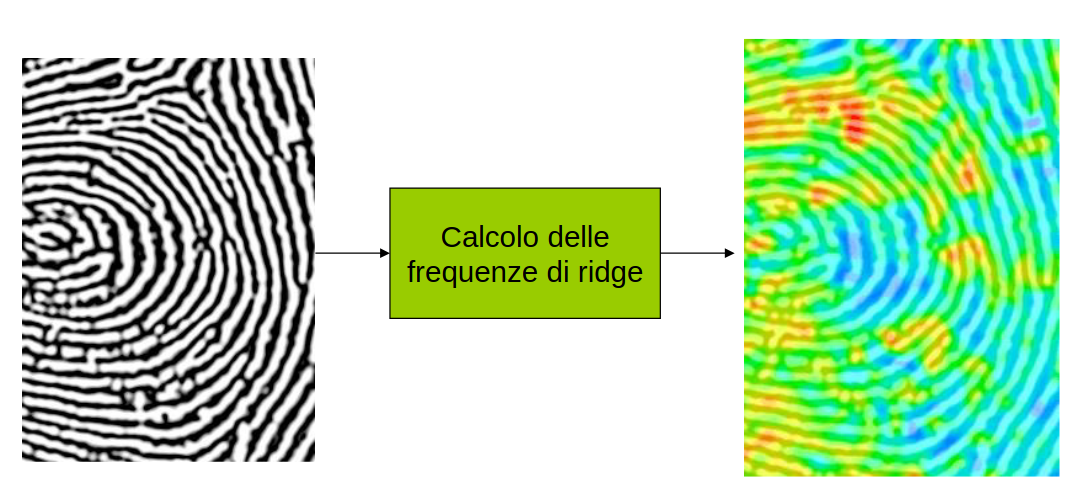
\includegraphics[width=1\linewidth]{images/spazio-freq.png}
\end{figure}

\newpage
\subsection{Core detection: metodo delle normali}

I punti di core possono essere calcolati utilizzando le normali.

\noindent Se seguendo N ridge e calcolando M normali abbiamo un numero sufficientemente
alto di intersezioni in un punto, allora abbiamo trovato un core.

\begin{figure}[ht]
    \centering
    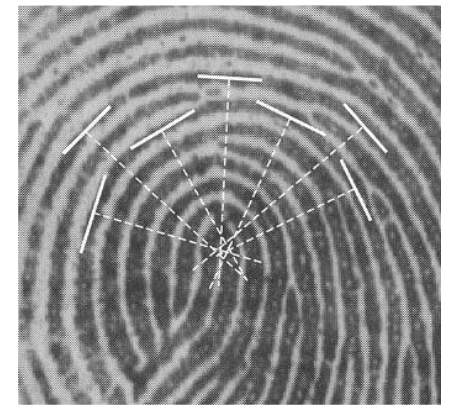
\includegraphics[width=0.5\linewidth]{images/core-detection.png}
\end{figure}

\section{Estrazione delle minuzie di II livello}

In questa sezione esaminiamo gli algoritmi per l'estrazione del II livello (minutiae).

\subsection{Metodi di binarizzazione}

I metodi di binarizzazione portano una immagine in toni di
grigio in una immagine in bianco e nero dove sono
evidenziati i ridge.

\subsection{Thinning}

L’operazione di thinning corrisponde ad ridurre
progressivamente le linee dell’immagine
binarizzata fino allo spessore di 1 pixel (scheletro
dell’immagine).

\begin{figure}[ht]
    \centering
    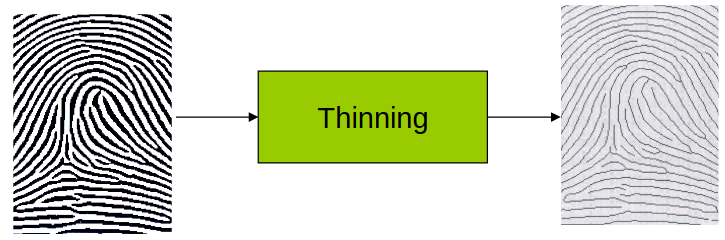
\includegraphics[width=0.75\linewidth]{images/thinning.png}
\end{figure}

\newpage
\noindent L’algoritmo deve anche (se possibile) riempire i
buchi nei ridge per non creare profili di questo
tipo:
\begin{figure}[ht]
    \centering
    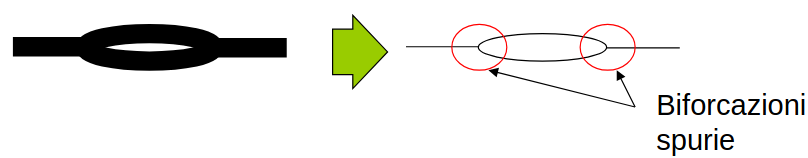
\includegraphics[width=1\linewidth]{images/thinning-bif.png}
\end{figure}


\subsection{Come identificare le minuzie}

Esaminando l’intorno di ogni punto lungo un ridge
di una immagine scheletrizzata è immediato capire in 
quale punto dell'impronta ci troviamo: basta contare le intersezioni
della matrice 3x3 attorno al punto.

\begin{figure}[ht]
    \centering
    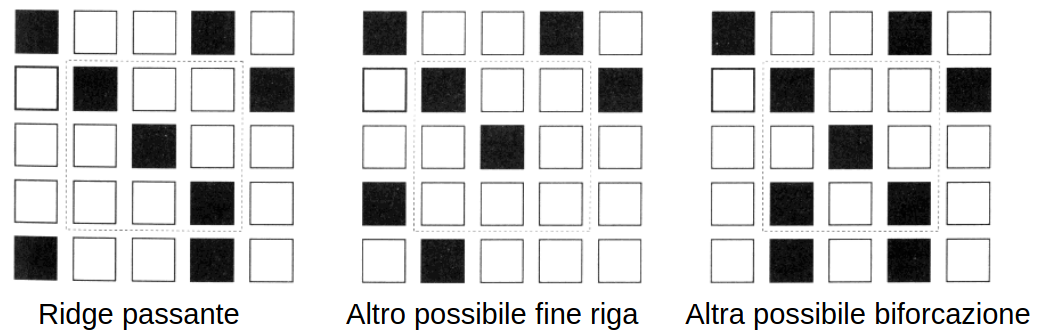
\includegraphics[width=1\linewidth]{images/identificazione-minuzie.png}
\end{figure}

\subsection{Metodi di post processing}

I moduli di post processing servono per rimuovere le
minutiae spurie introdotte dei moduli precedenti per errore.

\noindent L’errore che si può commettere è quello di togliere una
minutia corretta commettendo quindi errori.

\noindent Esistono due categorie principali di post processing:
\begin{itemize}
    \item structural post processing
    \item minutiae filtering in the gray-scale domain
\end{itemize}

\newpage
\subsubsection{Structural post processing}

Questi moduli sono tipicamente basati su regole che fanno riferimento
a caratteristiche dello scheeltro.

\begin{figure}[ht]
    \centering
    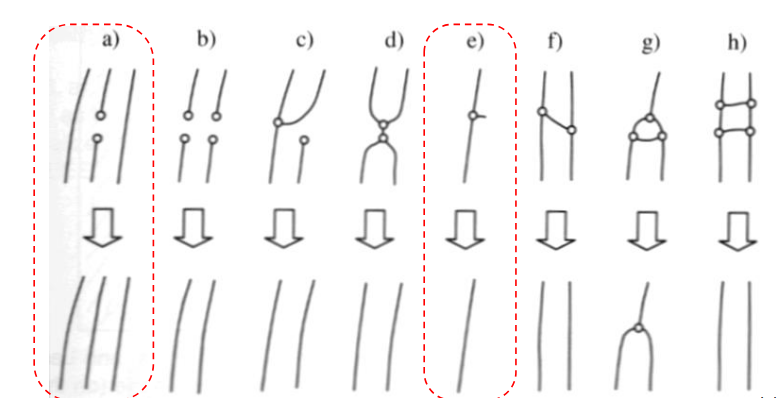
\includegraphics[width=0.75\linewidth]{images/structural-post.png}
\end{figure}

\section{Estrazione delle minuzie di III livello}

Nelle feature di III livello, tipicamente si studiano
le posizioni dei pori, attraverso le tecniche di segmentazione ed operatori morfologici.

\begin{figure}[ht]
    \centering
    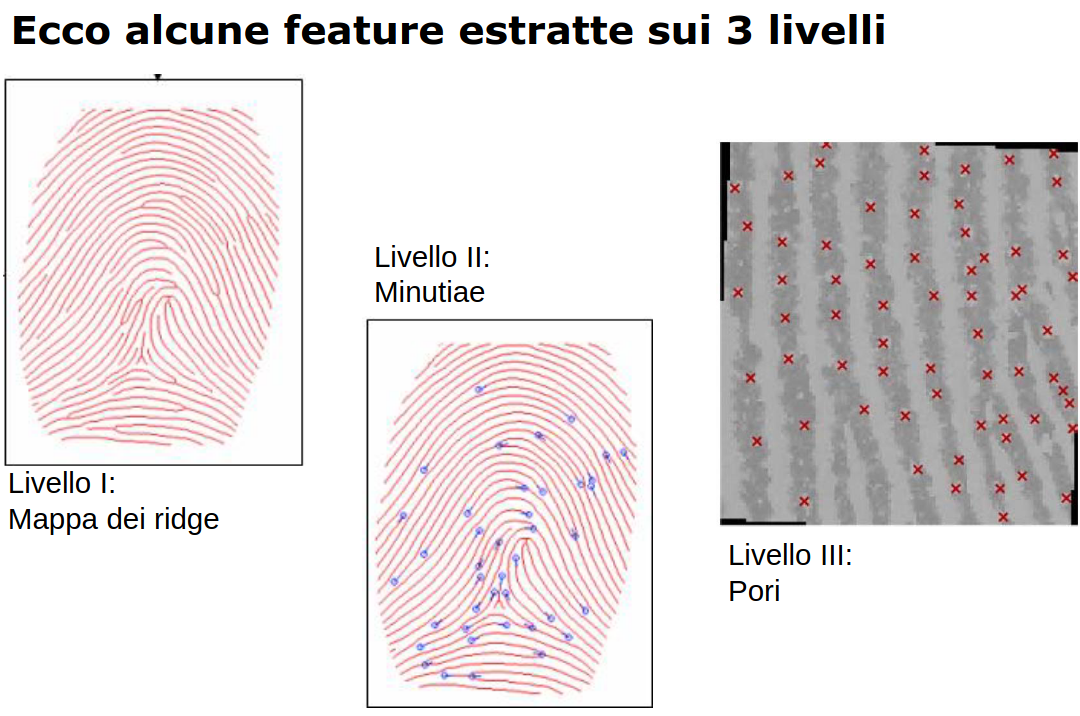
\includegraphics[width=1\linewidth]{images/es-conclusivo.png}
\end{figure}




\chapter{Spoofing e Anti-Spoofing}
Esistono molti modi per frodare un sistema biometrico:
\begin{itemize}
    \item attaccare i canali di comunicazione del sistema
    \item attaccare dei moduli specifici (ad esempio il modulo SW di estrazione delle caratteristiche)
    \item attaccare il DB con tutti i dati di enrollment
    \item ingannare il sensore, presentando un sample finto
\end{itemize}

\begin{figure}[ht]
    \centering
    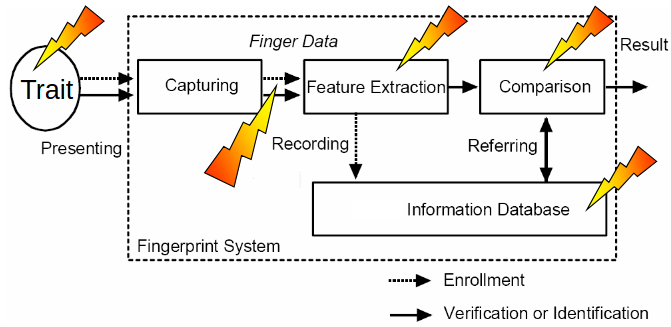
\includegraphics[width=0.75\linewidth]{images/frodare.png}
\end{figure}

\newpage
\section{Test di vitalità per sensori ottici}
Un metodo per effettuare anti-spoofing è quello di effettuare il test di vitalità:
consiste nell'usare uno o più segni vitali comuni a tutta la popolazione,
come ad esempio:
\begin{itemize}
    \item il \textbf{flusso sanguigno e la sua pulsazione}, che possono essere rilevati mediante la luce riflessa/trasmessa attraverso il dito 
    \item la \textbf{temperatura e la sua distribuzione}, in grado di indicare se il dito è vivo, morto o fasullo
    \item i \textbf{dettagli del III livello} rilevati da sensori ad alta risoluzione (>700 dpi), che sono difficili da imitare in un dito artificiale
    \item il \textbf{colore della pelle del dito}, che cambia colore per effetto della pressione
\end{itemize}

\noindent Inoltre, gli scanner ottici di tipo \textit{live-scan} o i sensori allo stato solido 
utilizzano un \textbf{meccanismo di acquisizione differenziata per le creste e i solchi} delle impronte, 
leggendo le differenze 3D dei ridge; in questo modo, sono in grado di difendersi
da attacchi che usano immagini 2D fasulle.

\section{Test di vitalità per sensori allo stato solido}
Le proprietà elettriche di un dito vivente possono essere facilmente 
misurate in un sensore a stato-solido, come ad esempio:
\begin{itemize}
    \item la \textbf{differenza di potenziale} tra due specifici punti della muscolatura del dito
    \item la \textbf{impedenza} del dito (resistenza di opposizione al passaggio della corrente elettrica)
    \item la \textbf{sudorazione}
\end{itemize}














\end{document}